%trust.tex
%%\nisarcomm{trim down to bare essentials, move rest of discussion/related work to the end...}

    %%In designing assurances that affect trust-based user behaviors, it is critical to know what drives those behaviors. Therefore, some time must be spent on understanding trust. 
    Trust is widely recognized as a critical part of %interpersonal relationships which affects 
    intelligent multi-agent system dynamics -- from those involving only simple one-on-one interactions \cite{Lewicki2006-hj} to more complex ones describing markets and governments \cite{Fukuyama1995-un}. 
    Because of interest spanning many disciplines, it is difficult (if not impossible) to write a succinct definition of trust that would completely satisfy all interested parties. 
    %Consequently, researchers in psychology, sociology, and economics have historically sought to understand the fundamental principles of trust~\cite{Gambetta1988-pi}. Moral philosophers have also thought intently about the topic \cite{Baier1986-im}. Because of interest spanning many disciplines, it is difficult (if not impossible) to write a succinct definition of trust that would completely satisfy all interested parties. %Besides that, trust is actually a very broad concept that evades concise definitions at a high level. However, the following adapted definition is broad enough to avoid too much contention \cite{McKnight2004-vv}:
    However, following \cite{McKnight2004-vv} for the purposes of this work, trust is defined here as a psychological state in which an agent willingly and securely becomes vulnerable, or depends on, a trustee (e.g., another person, institution, or an AIA), having taken into consideration the characteristics (e.g., benevolence, integrity, competence) of the trustee. 
%    \begin{description}
%        \item [Trust:] a psychological state in which an agent willingly and securely becomes vulnerable, or depends on, a trustee (e.g., another person, institution, or an AIA), having taken into consideration the characteristics (e.g., benevolence, integrity, competence) of the trustee.
%    \end{description}

%%    \subsubsection{A Model of Human-AIA Trust}
        This raises two important questions. Firstly, since trust is generally understood to exist between people, is it possible for a human to enter into a trusting relationship with an AIA? 
        That humans actually do develop trust in autonomous machines has been confirmed several times in research using common subjective psychological questionnaires~\cite{Muir1996-gt,Mcknight2011-gv,Riley1996-qm,Bainbridge2011-pl,Salem2015-md,Desai2012-rc, Freedy2007-sg, Kaniarasu2013-ho, Wang2016-id}. 
        %Several academic studies %experiments 
        %have also investigated the possibility of trust existing between humans and AIAs; %%(according to the terminology of this survey); 
        %all found that some level of trust can be formed in such relationships. 
        \citet{Lacher2014-yc} also points out that people trust AIAs for transportation systems at different levels. 
        %For instance, \citet{Lacher2014-yc} points out that people trust AIA at different levels.
        %As an example, an operator would have different perspectives on trust based on their level of interaction with the AIA. 
        %The designer of an AIA would also trust the AIA differently than an end user, due to the differing nature of the trust relationship from one to the other. 
        %%\citet{Tripp2011-rx} also concluded that, if a system is perceived to be `human enough', then a human trust model is appropriate. While there is technically a difference between their definitions of `human' and `system' trust we argue that, for practitioners, the differences are negligible. 
        %For instance, according to \cite{Tripp2011-rx}, the `competence' dimension of the human trust model described below can be replaced with one called `functionality', which has the same essential definition as competence, except that it accounts for reduced system complexity. Therefore, in the interest of simplicity we will use a human trust model as a basis for human-AIA trust -- with the understanding that the definitions of the model must correspondingly vary with the complexity of the AIA. It should be noted that this model is being presented as \emph{one possible model} that can be helpful in understanding assurances -- it is neither the only model nor a perfect model (as discussed above). As research advances, such models will likely continue to evolve, and the ideas of assurances will naturally evolve as well.
        %
        Secondly, in designing assurances that affect trust-based user behaviors, is it possible to know what drives those behaviors and thus have some working model of user trust that can be mapped to AIAs? 
        %%\citet{Tripp2011-rx} notes that, if a system is perceived to be `human enough', then a human trust model is appropriate. 
        %While there is technically a difference between their definitions of `human' and `system' trust 
        %Following \citet{Tripp2011-rx}, we argue that human-human trust models can be adopted here. %%%if an AIA is perceived to be `human enough'. 
        %, for practitioners, the differences are negligible, so that human-human trust models can be adapted here. 
        %In work relating to business management, 
        \citet{McKnight1998-ty} (and later \cite{McKnight2001-fa}) performed what is arguably the first multi-disciplinary survey and unification of trust literature, which also condensed it into a single typology consisting of three major related components. 
%       
        %The resulting model is shown, with some minor adaptations, in Figure~\ref{fig:UserTrust}. The figure illustrates the three components that make up a human's trust, with causal arrows that connect the different components. 
%
%       \begin{figure}[htbp]
%            \centering
%            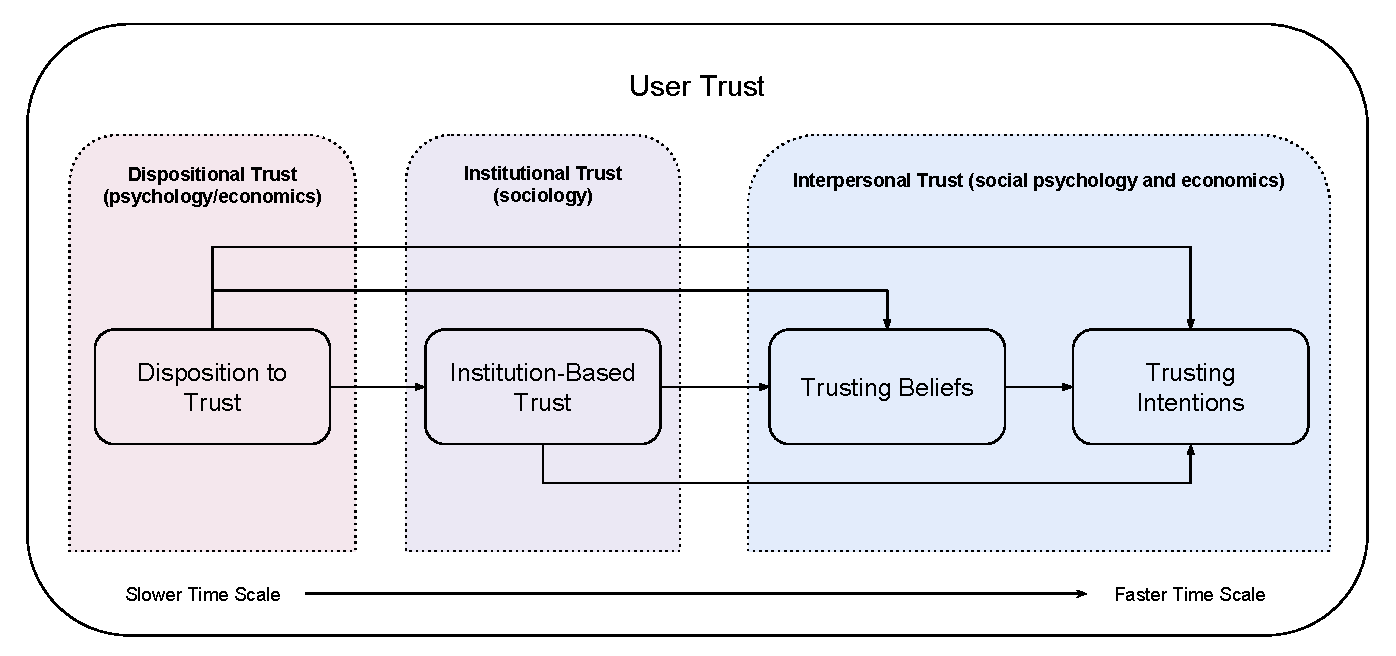
\includegraphics[width=0.6\textwidth]{Figures/UserTrust}
%            \caption{Depiction of interdisciplinary trust model proposed by \citet{McKnight2001-fa}.}
%            \label{fig:UserTrust}
%        \end{figure}
%
        %The categories in Figure~\ref{fig:UserTrust} 
        %
        Adapted to AIAs, these are: \textit{Disposition to Trust:} the extent to which one displays a tendency to be willing to depend on AIAs in general across a broad spectrum of situations and persons; \textit{Institution-Based Trust:} one believes that regulations are in place that are conducive to situational success in an endeavor; \textit{Trusting Beliefs:} one believes that the AIA has one or more characteristics beneficial to oneself; \textit{Trusting Intentions:} one is willing to depend on, or intends to depend on, the AIA even though one cannot control its every action. 
        Dispositional Trust is generally considered by psychologists, and deals with long-term psychological traits that develop in a person from childhood (e.g. is someone pre-disposed to trusting technology?).  
        Institutional Trust %(\brettcomm{ADD EXAMPLE ABOUT GOVERNMENT HERE, POSSIBLY REGULATIONS FOR THEME PARK RIDES}) 
        is generally studied by sociologists, and represents the level to which a person trusts social/commercial structures. 
        Finally, Interpersonal Trust deal directly with one-on-one relationships and tend to fluctuate most quickly. 
        Each of these trust components has sub-components defined in Figure~\ref{fig:Assurance_classes}, which were identified by compiling many research studies across research disciplines. 
        These components are the principal drivers of user trust-related behaviors, and are the general notional targets of AIA assurances.

        \begin{figure}[t]%[htbp]
            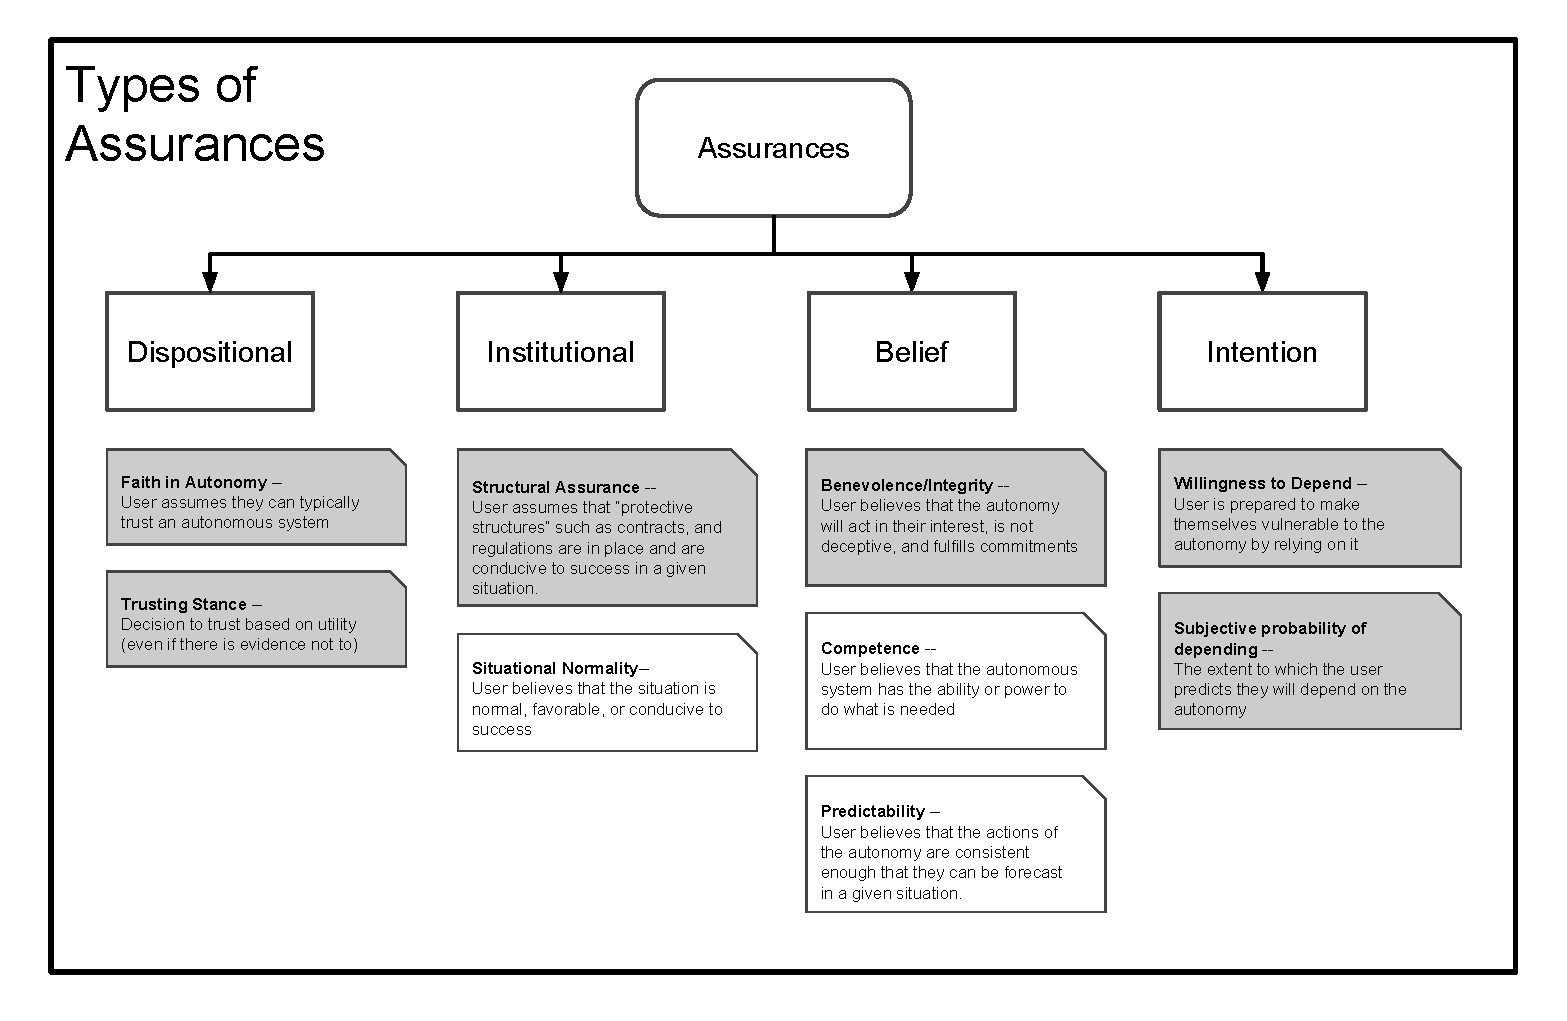
\includegraphics[width=0.95\textwidth]{Figures/Assurances.pdf}%
            \caption{Notional assurance targets based on the component definitions of the main categories of trust.}
            \label{fig:Assurance_classes}
        \end{figure}
